%===========================================================
% 05_development.tex - 开发指导
%===========================================================

\section{开发指导}

\begin{frame}{开发环境搭建}
    \begin{block}{步骤1:创建项目目录}
        \begin{center}
            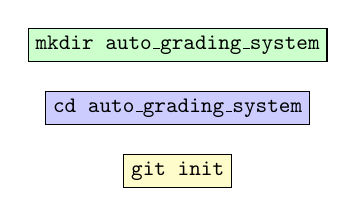
\begin{tikzpicture}[scale=0.8, transform shape]
                \node[draw, rectangle, fill=green!20] at (0,0) {\texttt{mkdir auto\_grading\_system}};
                \node[draw, rectangle, fill=blue!20] at (0,-1) {\texttt{cd auto\_grading\_system}};
                \node[draw, rectangle, fill=yellow!20] at (0,-2) {\texttt{git init}};
            \end{tikzpicture}
        \end{center}
    \end{block}

    \begin{block}{步骤2:创建虚拟环境}
        \texttt{python -m venv venv}\\
        \texttt{source venv/bin/activate}  \# Linux/Mac\\
        \texttt{venv\Scripts\activate}     \# Windows
    \end{block}

    \begin{block}{步骤3:安装依赖}
        \texttt{pip install opencv-python paddlepaddle paddleocr numpy pillow matplotlib}
    \end{block}

    \begin{block}{步骤4:创建项目结构}
        \texttt{mkdir -p modules utils data/\{input,output,templates,test\}}
    \end{block}
\end{frame}

\begin{frame}{项目目录结构}
    \begin{block}{智能阅卷系统完整结构}
        \begin{center}
            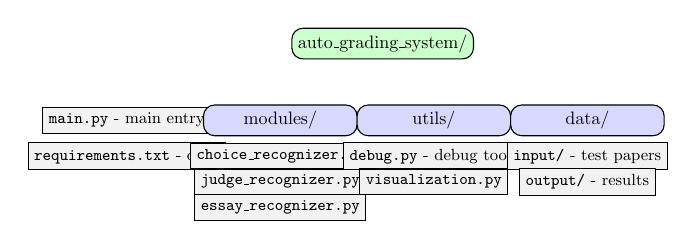
\begin{tikzpicture}[scale=0.65, transform shape,
                dir/.style={draw, rectangle, rounded corners, fill=blue!15, minimum width=3cm, minimum height=0.6cm, align=center},
                file/.style={draw, rectangle, fill=gray!10, minimum width=2.5cm, minimum height=0.5cm, align=left, font=\small},
                arrow/.style={->, thick}]

                \node[dir, fill=green!20] (root) at (5,3) {auto\_grading\_system/};

                \node[file] (main) at (0,1.5) {\texttt{main.py} - main entry};
                \node[file] (req) at (0,0.8) {\texttt{requirements.txt} - deps};

                \node[dir] (modules) at (3,1.5) {modules/};
                \node[file] (choice) at (3,0.8) {\texttt{choice\_recognizer.py}};
                \node[file] (judge) at (3,0.3) {\texttt{judge\_recognizer.py}};
                \node[file] (essay) at (3,-0.2) {\texttt{essay\_recognizer.py}};

                \node[dir] (utils) at (6,1.5) {utils/};
                \node[file] (debug) at (6,0.8) {\texttt{debug.py} - debug tools};
                \node[file] (viz) at (6,0.3) {\texttt{visualization.py}};

                \node[dir] (data) at (9,1.5) {data/};
                \node[file] (input) at (9,0.8) {\texttt{input/} - test papers};
                \node[file] (output) at (9,0.3) {\texttt{output/} - results};
            \end{tikzpicture}
        \end{center}
    \end{block}
    \begin{alertblock}{Course Materials}
        utils/debug.py and utils/visualization.py are provided (70\% framework code)
    \end{alertblock}
\end{frame}

\section{Debug Tools}

\begin{frame}{Debug Tools: save\_debug\_image}
    \textbf{Function: save\_debug\_image(image, name, output\_dir="debug")}

    \begin{block}{Purpose: Save debug images for troubleshooting}
        \begin{itemize}
            \item Creates output directory automatically
            \item Adds timestamp to filename for uniqueness
            \item Saves as PNG format
        \end{itemize}
    \end{block}

    \textbf{Usage Example:}
    \begin{center}
        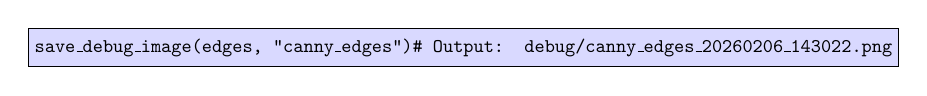
\begin{tikzpicture}[scale=0.7, transform shape]
            \node[draw, rectangle, fill=blue!15, minimum width=10cm, minimum height=0.7cm] {
                \texttt{save\_debug\_image(edges, "canny\_edges")}\\
                \texttt{\# Output: debug/canny\_edges\_20260206\_143022.png}
            };
        \end{tikzpicture}
    \end{center}
\end{frame}

\begin{frame}{Debug Tools: draw\_debug\_boxes}
    \textbf{Function: draw\_debug\_boxes(image, boxes, labels, color)}

    \begin{block}{Purpose: Visualize detection results on images}
        \begin{itemize}
            \item Draws bounding boxes on the image
            \item Optional labels for each box
            \item Customizable BGR color
        \end{itemize}
    \end{block}

    \textbf{Usage Example:}
    \begin{center}
        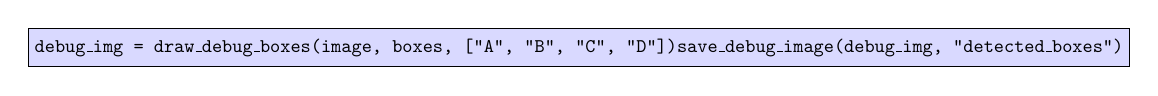
\begin{tikzpicture}[scale=0.7, transform shape]
            \node[draw, rectangle, fill=blue!15, minimum width=10cm, minimum height=0.7cm] {
                \texttt{debug\_img = draw\_debug\_boxes(image, boxes, ["A", "B", "C", "D"])}\\
                \texttt{save\_debug\_image(debug\_img, "detected\_boxes")}
            };
        \end{tikzpicture}
    \end{center}
\end{frame}

\begin{frame}{Debug Tools: DebugPipeline Class}
    \textbf{Class: DebugPipeline - Pipeline Step Visualization}

    \begin{block}{Key Methods:}
        \begin{itemize}
            \item \texttt{\_init\_(output\_dir="debug")} - Initialize with output directory
            \item \texttt{add\_step(name, image, info)} - Add processing step
            \item \texttt{save\_all\_steps()} - Save all step images
            \item \texttt{visualize()} - Display all steps in windows
        \end{itemize}
    \end{block}

    \textbf{Usage Example:}
    \begin{center}
        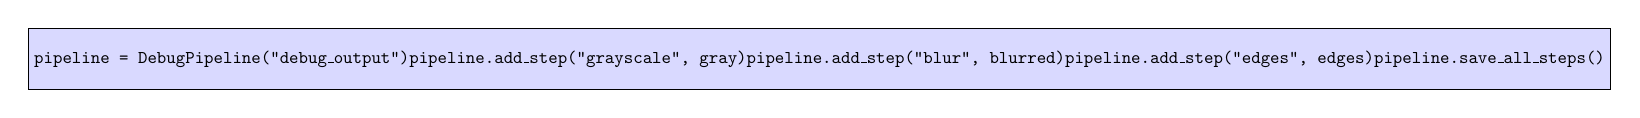
\begin{tikzpicture}[scale=0.65, transform shape]
            \node[draw, rectangle, fill=blue!15, minimum width=10cm, minimum height=1.2cm] {
                \texttt{pipeline = DebugPipeline("debug\_output")}\\
                \texttt{pipeline.add\_step("grayscale", gray)}\\
                \texttt{pipeline.add\_step("blur", blurred)}\\
                \texttt{pipeline.add\_step("edges", edges)}\\
                \texttt{pipeline.save\_all\_steps()}
            };
        \end{tikzpicture}
    \end{center}
\end{frame}

\section{Interface Design}

\begin{frame}{Module Interface Standard}
    \textbf{Recognizer Interface Definition:}

    \begin{center}
        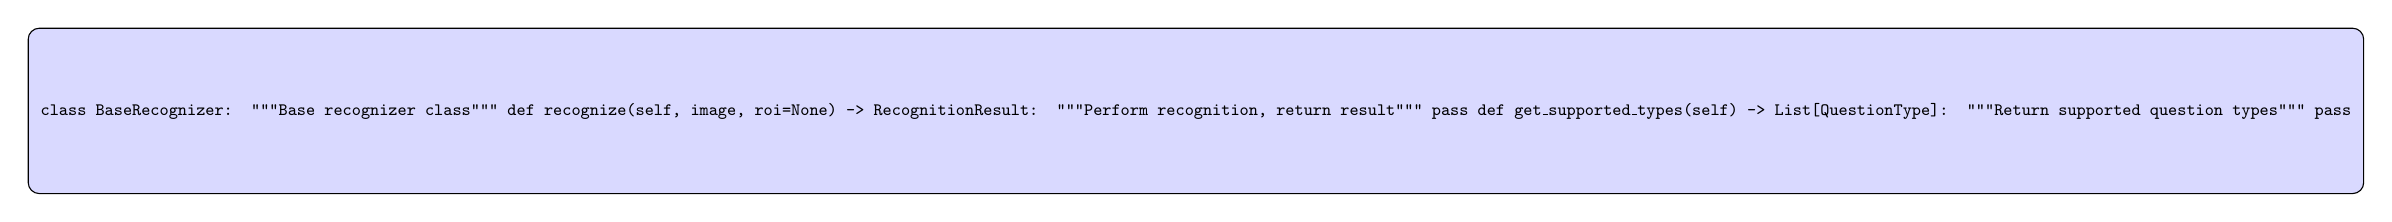
\begin{tikzpicture}[scale=0.7, transform shape]
            \node[draw, rectangle, fill=blue!15, minimum width=10cm, minimum height=3cm, rounded corners] {
                \begin{small}
                \texttt{class BaseRecognizer:}\\
                \texttt{    """Base recognizer class"""}\\
                \texttt{    }\\
                \texttt{    def recognize(self, image, roi=None) -> RecognitionResult:}\\
                \texttt{        """Perform recognition, return result"""}\\
                \texttt{        pass}\\
                \texttt{    }\\
                \texttt{    def get\_supported\_types(self) -> List[QuestionType]:}\\
                \texttt{        """Return supported question types"""}\\
                \texttt{        pass}
                \end{small}
            };
        \end{tikzpicture}
    \end{center}

    \begin{alertblock}{Interface Contract}
        \begin{itemize}
            \item Input: image (numpy.ndarray) or ROI region
            \item Output: RecognitionResult (text, confidence, question\_type)
            \item Exception: Return result with confidence=0, no exceptions
        \end{itemize}
    \end{alertblock}
\end{frame}

\begin{frame}{RecognitionResult Data Structure}
    \textbf{Data Structure Definition:}

    \begin{center}
        \begin{tikzpicture}[scale=0.7, transform shape]
            \node[draw, rectangle, fill=green!15, minimum width=10cm, minimum height=3.5cm, rounded corners] {
                \begin{small}
                \texttt{class RecognitionResult:}\\
                \texttt{    def \_\_init\_\_(self, text, confidence, question\_type):}\\
                \texttt{        self.text = text              \# Recognized text content}\\
                \texttt{        self.confidence = confidence  \# 0.0-1.0, recognition confidence}\\
                \texttt{        self.question\_type = type    \# QuestionType enum}\\
                \texttt{        self.bounding\_box = None     \# Optional: ROI coordinates}\\
                \texttt{        self.metadata = \{\}          \# Optional: extra info}\\
                \texttt{    }\\
                \texttt{    def is\_valid(self) -> bool:}\\
                \texttt{        """Check if result is valid for grading"""}\\
                \texttt{        return self.confidence > 0.6}
                \end{small}
            };
        \end{tikzpicture}
    \end{center}
\end{frame}
